\documentclass[11pt]{article}

\usepackage[margin=1in]{geometry}
\usepackage{graphicx}
\usepackage[colorlinks=true,allcolors=blue]{hyperref}
\usepackage{authblk}
\usepackage[style=numeric, sorting=none, backend=biber]{biblatex}
\addbibresource{references.bib}



% determines the spacing and general formatting of each section in the document
\makeatletter
\renewcommand{\@maketitle}{%
    \newpage
    \null
    \vskip 2em%
    \let\footnote\thanks
    \begin{center}%
        {\LARGE \@title \par}%
    \end{center}%
        \vskip 1em%
        {\large \noindent\begin{minipage}{\textwidth}\raggedright \@author\end{minipage}\par}%
        \vskip 1em%
    \begin{center}%
        {\@date}%
    \end{center}%
    \par
    \vskip 1.5em%
}

% Compact bibliography format: [N] Author et al., Year, ShortJournal.
\DeclareNameFormat{familyonly}{%
  \ifnumequal{\value{listcount}}{1}{%
    \namepartfamily%
    \ifnumgreater{\value{listtotal}}{1}{ et al.}{}%
  }{}%
}
\DeclareBibliographyDriver{article}{%
  \printnames[familyonly]{author}%
  , \printfield{year}%
  , \printfield{shortjournal}%
  }
\DeclareBibliographyDriver{inproceedings}{%
  \printnames[familyonly]{author}%
  , \printfield{year}%
  , \printfield{shortjournal}%
}
\AtBeginBibliography{\setlength{\parskip}{0pt}}
\setlength{\bibitemsep}{0pt}
\setlength{\bibparsep}{0pt}

\makeatother

\title{The Consequences of an Icy Porous Layer on the Thermal State and Radar Attenuation of Enceladus' Ice Shell}
\renewcommand\Authands{, }
\author[1,2]{William Byrne}
\author[1]{Ana-Catalina Plesa}
\author[1]{Tina Ruckriemen-Bez}
\author[3]{Andreas Benedikter}
\author[1]{Hauke Hussmann}


\affil[1]{Institute of Space Research, German Aerospace Center (DLR), Berlin, Germany\\
\href{mailto:William.Byrne@dlr.de}{William.Byrne@dlr.de}; \href{mailto:Ana.Plesa@dlr.de}{Ana.Plesa@dlr.de}; \href{mailto:tina.rueckriemen-bez@dlr.de}{tina.rueckriemen-bez@dlr.de}; \href{mailto:Hauke.Hussmann@dlr.de}{Hauke.Hussmann@dlr.de};}
\affil[2]{University of Maryland, College Park, MD, USA\\
\href{mailto:wbyrne@umd.edu}{wbyrne@umd.edu}}
\affil[3]{Microwaves and Radar Institute, German Aerospace Center (DLR), Weßling, Germany\\
\href{mailto:Andreas.Benedikter@dlr.de}{Andreas.Benedikter@dlr.de}}
\date{03.07.2024:
\href{https://doi.org/10.5194/epsc2024-694}{View abstract on the EPSC2024 website}}

\begin{document}

\maketitle

\raggedright
\setlength{\parindent}{0pt}
\setlength{\parskip}{\baselineskip}

\section*{Abstract}

Saturn's moon, Enceladus is considered a priority target for future planetary missions due to its high astrobiological potential \parencite{choblet2021enceladus}. Water jets presumably originating from a subsurface ocean have been observed at the south pole of Enceladus by NASA’s Cassini mission \parencite{hansen2006enceladus}, and their analysis provides a direct window into the ocean composition \parencite{postberg2009sodium} that, in turn, can help to understand the nature and amount of impurities that may exist within the ice shell.
 
Enceladus’ jet activity generates a highly porous material that affects the thermal state of the ice shell. The thickness of that layer and its distribution are poorly constrained, but local thicknesses of up to 700 m have been reported from the analysis of pit chains on the surface of Enceladus \parencite{martin2023}. Such a thick porous layer can strongly attenuate the signal of radar sounders that have been proposed to investigate the Enceladus’ subsurface \parencite{soucek2023}.

Here, we use numerical simulations to determine the effects of a porous layer on the two-way radar attenuation. We generate a variety of steady-state one-dimensional thermal models based on proposed parameters for Enceladus’ ice shell thickness (5 - 35 km, \parencite{hemingway2019enceladus}), porous layer thickness (0 - 700 m \parencite{martin2023}) and its thermal conductivity (0.1 - 0.001 W/mK \parencite{seiferlin1996,ferrari2021}). We define a penetration depth, which is the depth at which the two-way attenuation reaches a 100 dB, a typical value for radar sounders on planetary missions\parencite{kalousova17}. We use two material models ("high" and "low" loss) to identify the impact of chemical impurities on attenuation\parencite{kalousova17}. While the “low” loss scenario considers an ice shell composed of pure water ice, the “high” loss case is characterized by a homogeneous mixture of water ice and chlorides in concentrations extrapolated from the particle composition of Enceladus’ plume \parencite{soucek2023}.

\begin{figure}[htbp]
\noindent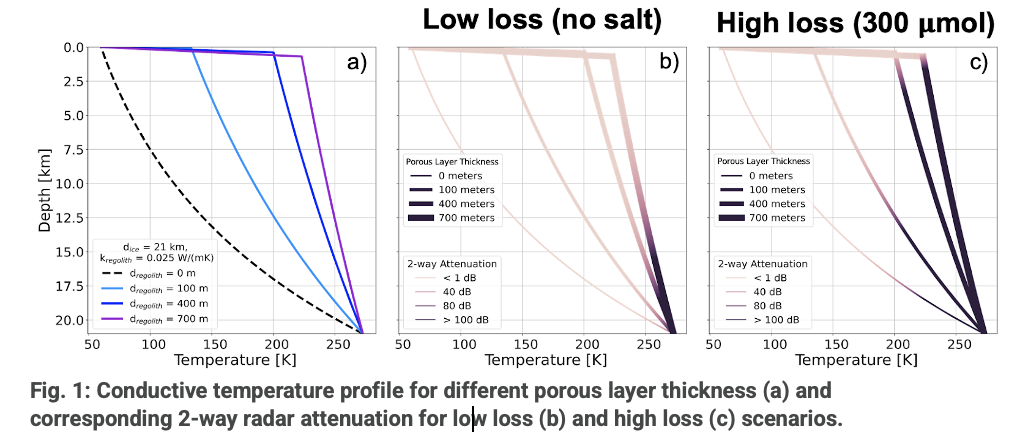
\includegraphics[width=\textwidth]{poster_figures/EPSC2024/fig1_epsc2024.png}
\label{fig1}
\end{figure}

For a conductive ice shell, the temperature itself depends on the thickness of the ice shell, and to a first order on the presence of a porous layer. Due to its insulating effect caused by its low thermal conductivity, the porous layer can significantly impact the thermal profile within the ice shell, leading to a high thermal gradient near the surface. We can clearly observe in Figure 1 that the attenuation dramatically increases with increasing porous layer thickness. This can be again attributed to the insulating effect of the porous layer, an effect that becomes more pronounced with increasing porous layer thickness. 

\begin{figure}[htbp]
\noindent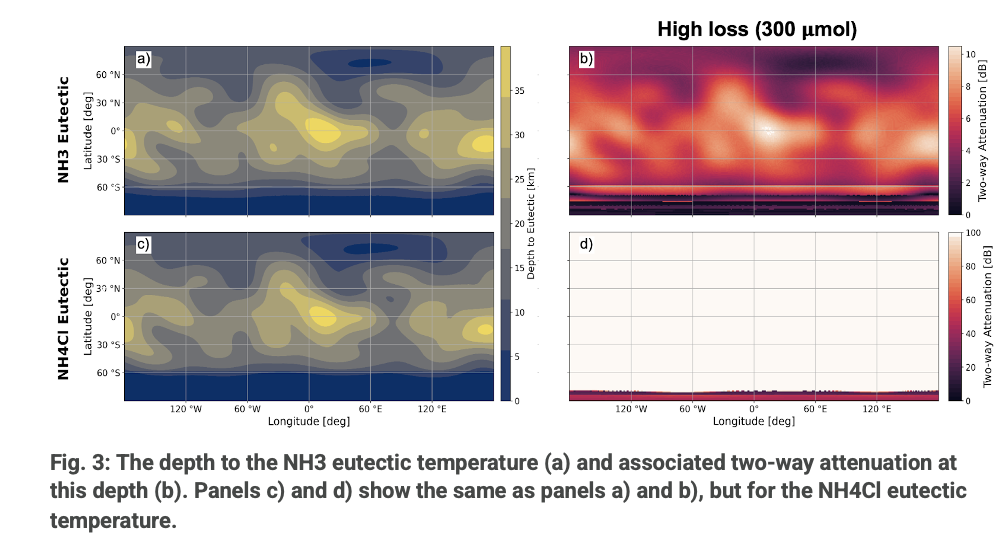
\includegraphics[width=\textwidth]{poster_figures/EPSC2024/fig2_epsc2024.png}
\label{fig2}
\end{figure}

In addition to systematically testing parameter combinations, we use two ice shell thickness maps \parencite{hemingway2019enceladus} together with local thermal profiles to provide a global spatial distribution of potential penetration depths that could be achieved by radar measurements. The attenuation was calculated by treating each data point as a single temperature profile using the corresponding ice shell thickness at the respective location. We define a penetration depth, which is the depth at which the two-way attenuation reaches 100 dB. The relative penetration depth is the penetration depth divided by the total ice shell thickness of the respective scenario. 

We constructed two distribution models for the porous layer under the assumption that the thickness of the porous layer varies only with latitude and: 1) exponentially decreases from a 700-m-thick layer at the south pole to 10-m-thick layer at the north pole of Enceladus, which we denote as the "exponential-global distribution" (see figure 2d) while 2) the porous layer is absent within the 5° of the south pole and then exponentially decreases from 255 m to 0 m at equator (see figure 2g), which we will call "exponential-hemispheric distribution". In all cases the conductivity of the porous layer is 0.025 Wm-1K-1. 

In the low-loss attenuation maps (Figure 2d, e, and f), a majority of the surface has more than 90% relative penetration depth, while in all three high-loss scenarios, we observe a small band of 100% relative penetration depth roughly 5° in latitude away from the south pole. The thin ice shell at the south pole allows for the signal to reach the ice-ocean interface even in the presence of a thick porous layer. 

\begin{figure}[htbp]
\noindent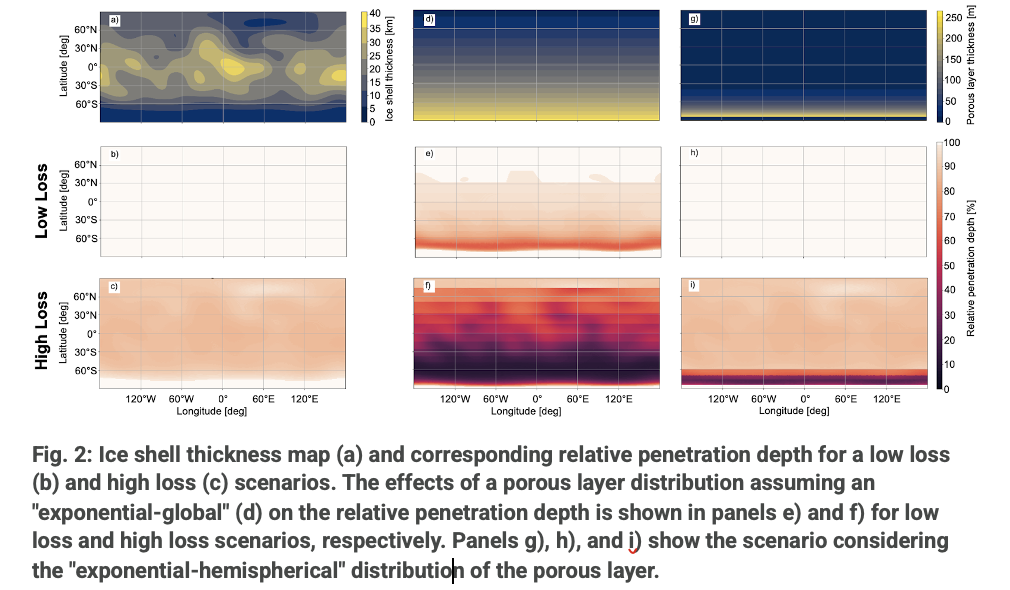
\includegraphics[width=\textwidth]{poster_figures/EPSC2024/fig3_epsc2024.png}
\label{fig3}
\end{figure}

In Figure 3, we calculate the two-way attenuation at the eutectic interfaces of ammonium chloride and ammonia \parencite{soucek2023} for the exponential-hemispheric distribution of the porous layer and assuming a thermal conductivity of the porous layer of 0.025 W/(mK). 

Given the low eutectic temperature of NH3 (175.45 K), the two-way attenuation for the high-loss case (Figure 3b) is only ~5 dB on average. For the eutectic interface of NH4Cl (257.79 K), the two-way attenuation shows an average value of about 400 dB (Figure 3d). 
 
In conclusion, our results show that the presence of a porous layer has a first-order effect on the two-way radar attenuation. For regions covered by porous layers with thicknesses larger than 250 m and a thermal conductivity lower than 0.025 W/(mK) the two-way radar attenuation reaches a threshold value of 100 dB before reaching the ice-ocean interface in the low loss scenarios. In the high loss cases, for similar regolith layer thicknesses and thermal conductivity, the two-way attenuation remains below 100 dB for at most 48% of the ice shell. Depending on the local ice shell thickness and properties of the snow deposits, as little as a few percent of the ice shell can be penetrated before the 100 dB limit is reached. We note, however, that the presence of a porous layer leads to high subsurface temperatures and promotes the formation of brines at shallow depth that can be detected by future radar measurements.


\printbibliography[title={References}]

\end{document}
